\section{ХОД РАБОТЫ}

\subsection{Формулировка задачи}

Требуется выполнить моделирование простейшего потока событий
приведенными в подразделе~\ref{subs:theory} алгоритмами. Вывести графическую
иллюстрацию потоков в виде нанесения на ось абсцисс моментов появления
требований и концов промежутка $(a,b)$. Параметры потока для моделирования:
\begin{equation*}
  \lambda = 6, \hspace{5mm} a = 0, \hspace{5mm} b = 50.
\end{equation*}

Вывести гистограмму промежутка времени между соседними требованиями потока
и его плотность вероятности. Для согласования масштабов гистограммы и генеральной
плотности вероятности необходимо генеральную плотность вероятности умножить на
коэффициент $k$:
\begin{equation}
\label{eq:k}
  k = n \dfrac{\Delta_{(n)} - \Delta_{(1)}}{l}.
\end{equation}

В выражении~\ref{eq:k} имеем: $n$ --- объём выборки, $l$ --- число интервалов разбиения
выборки при построении гистограммы, $ \Delta_{(n)}, \Delta_{(n)} $ ---
минимальный и максимальный из интервалов времени между требованиями соответственно.

Кроме этого, требуется получить оценку $\overline{\lambda}$ параметра $\lambda$ потока. 


\subsection{Теоретические сведения}
\label{subs:theory}

Потоком однородных событий (требований) называется конечная или счетная
последовательность $\tau_n$ случайных величин, определённых на одном и том же
вероятностном пространстве, при условии, что любой фиксированный интервал времени
$(a,b)$ с вероятностью 1 попадает конечное число этих величин.

Поток требований в системе массового обслуживания (СМО) называется простейшим
или Пуассоновским, если он обладает свойствами стационарности, ординарности,
отсутствия последействия.

\textit{Стационарность} потока означает, что для любой группы из конечного числа $n$
непересекающихся отрезков времени вероятность появления в них соответственно
$ k_1, k_2, ..., k_n $ требований зависит только от этих чисел и длин указанных
промежутков времени, но не зависит от их расположения на оси времени. В частности,
вероятность $p_k$ появления $k$ требований на отрезке $[T, T+t]$ не зависит от
$T$ и является функцией только $k$ и $t$: $p_k = p_k(k,t)$.

\textit{Ординарность} потока означает практическую невозможность появления двух или более
требований в один и тот же момент времени. В математической форме ординарность
записывается следующим образом:
\begin{equation}
  \dfrac{p_{>1}(h)}{h} \rightarrow 0, \text{  при } h \rightarrow 0,
\end{equation}
\par где $p_{>1}(h)$ --- вероятность появления на отрезке длиной $h$ двух и более
требований. Отсюда сразу следует, что для простейшего потока $p_{>1}(0) = 0$.

\textit{Отсутствие последействия} состоит в том, что вероятность поступления $k$
требований в течение отрезка времени $[T,T+t]$ не зависит от того, сколько требований
и как поступали до этого отрезка. Иначе говоря, количества требований (случайные
величины), поступающие в непересекающиеся отрезки времени, независимы в совокупности.

Рассмотрим алгоритмы моделирования простейшего потока заявок.

\textit{Алгоритм 1.}

\begin{enumerate}
  \item Определяем интервал $(a, b)$, параметр $\lambda$.
  \item Моделируем независимые последовательные интервалы времени $\Delta_1 =
    \tau_1 - a$, $\Delta_2 = \tau_2 - \tau_1, ...$, распределённые по
    экспоненциальному закону с параметром $\lambda$, до тех пор,
    пока $\tau_m = a + \sum\limits_{i=1}^{m}\Delta_i \le b $, $ m=1,2,... $, $\tau_0 = a$.
    Величины $\tau_1, \tau_2,... $ здесь являются моментами появления
    заявок. Их число заранее не определено.
\end{enumerate}

\textit{Алгоритм 2.}

\begin{enumerate}
  \item Определяем интервал $(a, b)$, параметр $\lambda$.
  \item Моделируем число заявок $n$ потока как случайное число из пуассоновского
    распределения $\text{П}(\lambda (b-a))$.
  \item Моделируем $n$ независимых случайных чисел $z_1, z_2, ..., z_n$ из
    равномерного в $(a,b)$ распределения.
  \item Сортируем случайные числа $ z_1, z_2, ..., z_n $ в порядке возрастания,
    в результате чего получаем последовательные моменты
    времени $ \tau_1, \tau_2, ..., \tau_n$ поступления заявок.
  \item Рассчитываем интервалы времени между заявками $ \Delta_1 =
    \tau_1 - a, \Delta_2 = \tau_2 - \tau_1, ..., \Delta_n = \tau_n - \tau_{n-1} $.
\end{enumerate}

\subsection{Ход работы}

Выполним моделирование реализаций простейшего потока двумя приведенными
в подразделе~\ref{subs:theory} алгоритмами. На рисунке~\ref{pic:times} приведена
иллюстрация пуассоновского потока, построенного по алгоритмам 1 и 2.

\begin{figure}[h!]
  \centering
  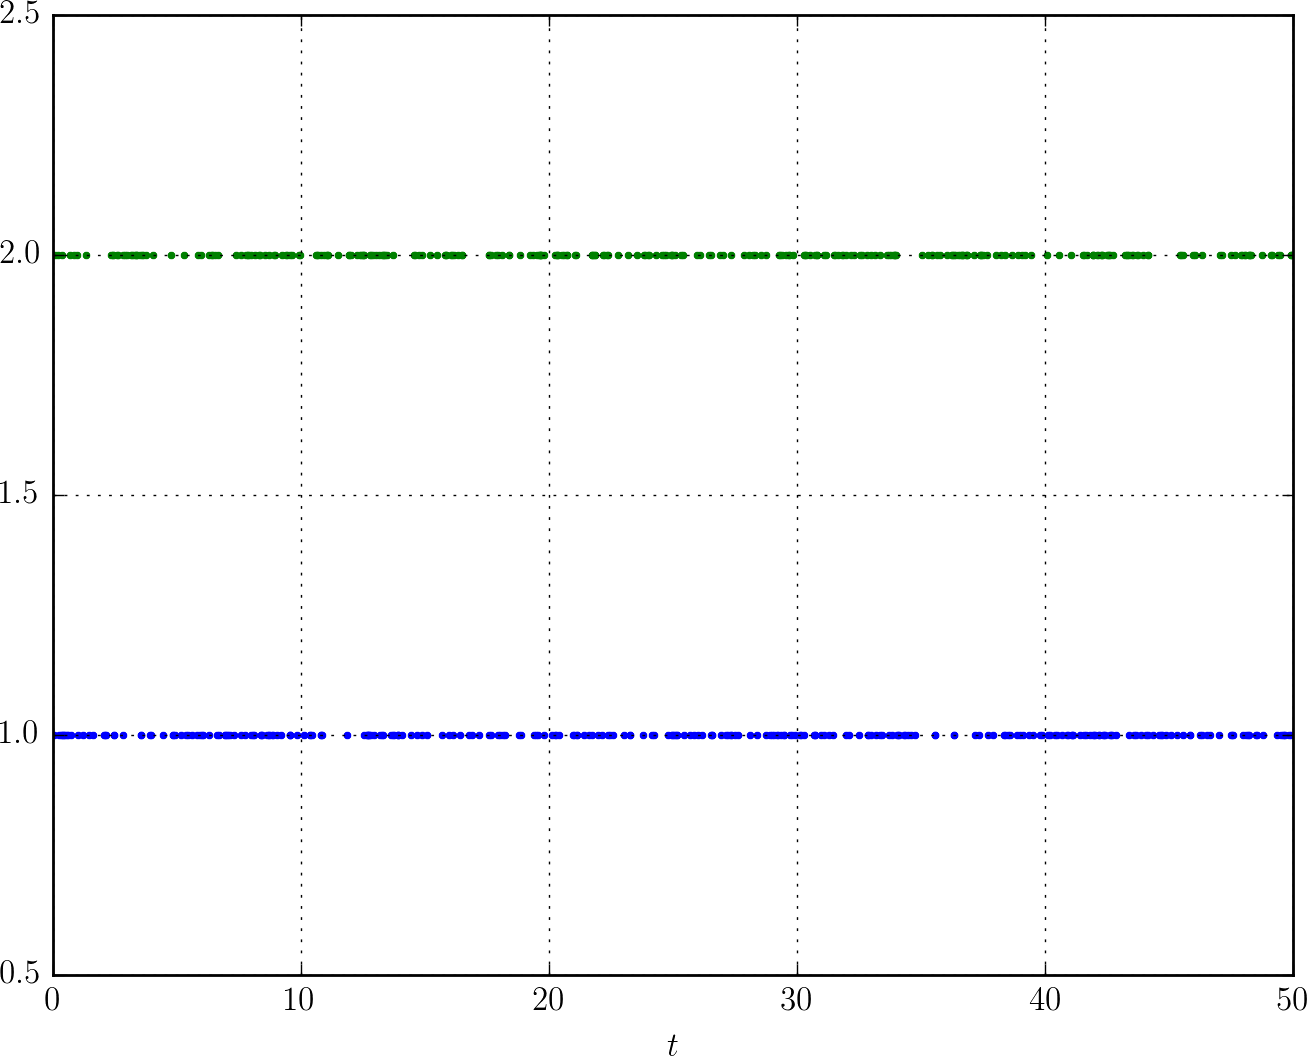
\includegraphics[width=150mm, height=85mm]{pic/times}
  \caption{Иллюстрация пуассоновского потока, построенного по алгоритмам 1 и 2}
  \label{pic:times}
\end{figure}

На рисунках~\ref{pic:hist_1}~и~\ref{pic:hist_2} приведены гистограммы и плотности вероятности распределения промежутков времени между соседними заявками пуассоновского потока в СМО.

\begin{figure}[h!]
  \centering
  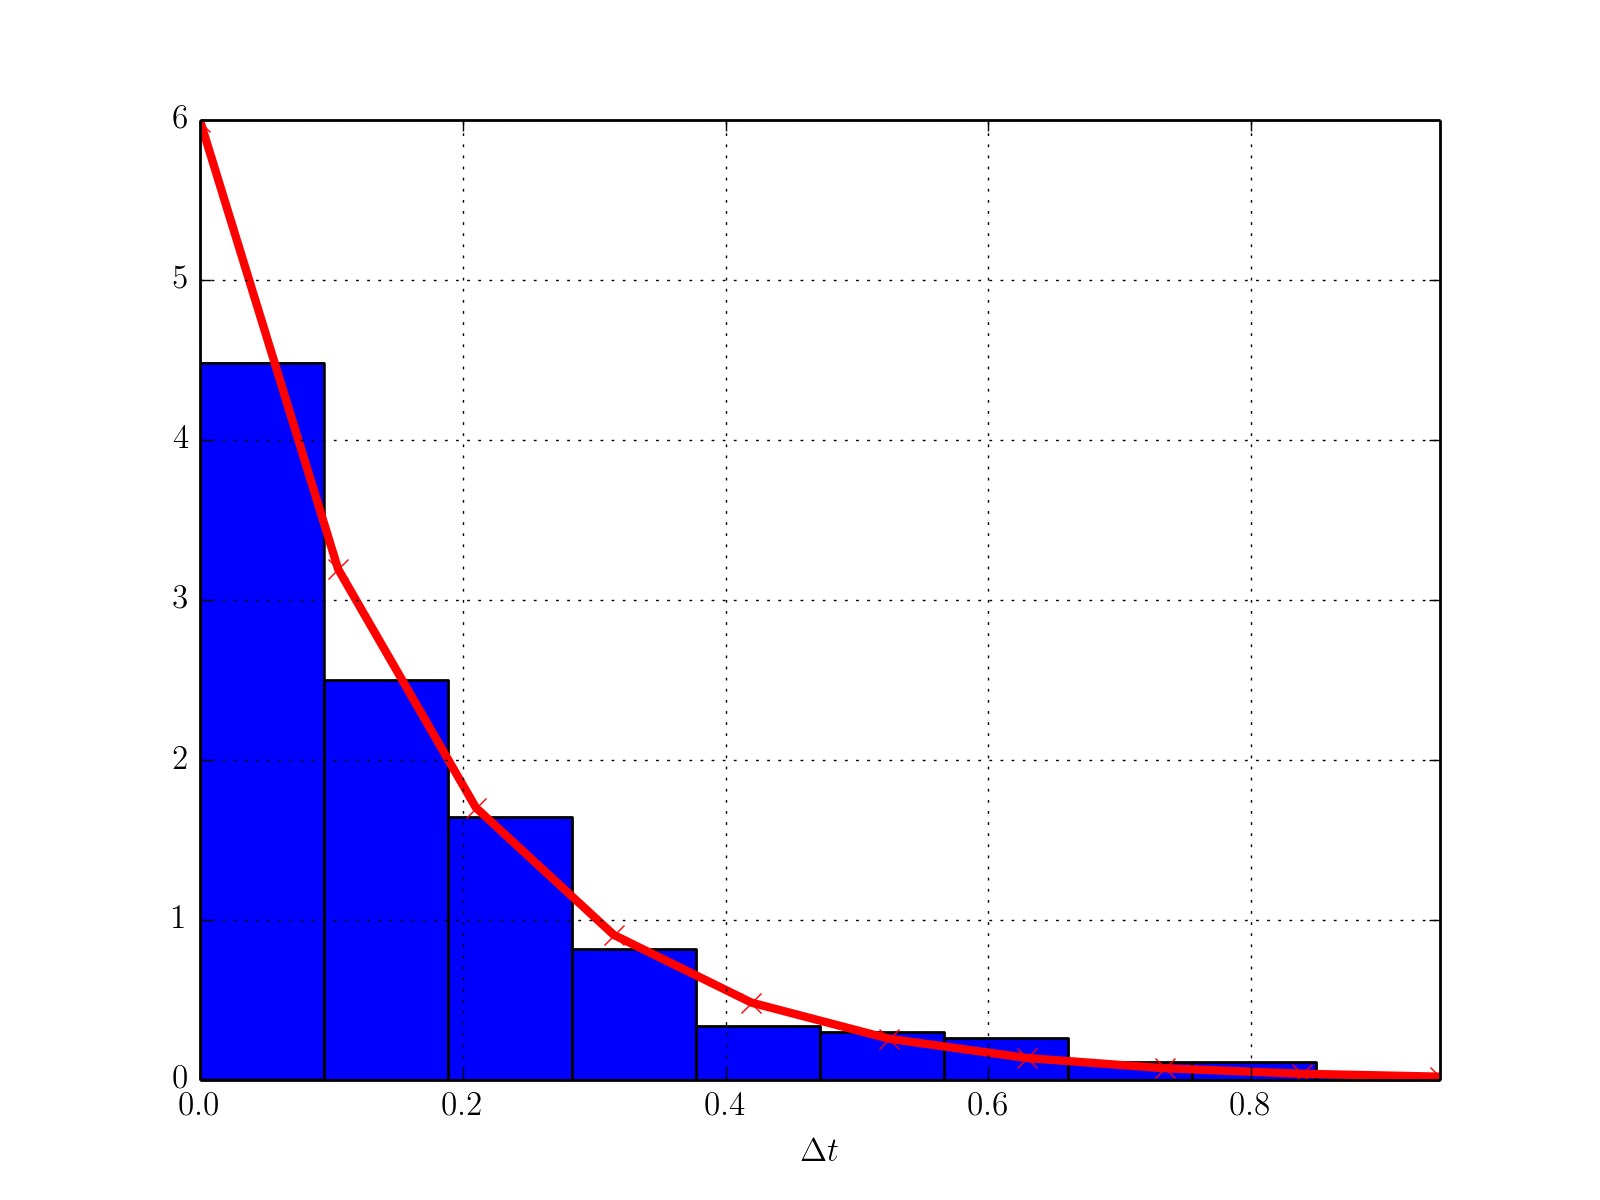
\includegraphics[width=150mm, height=85mm]{pic/hist_1}
  \caption{Гистограмма и плотность вероятности промежутков времени
    между соседними заявками пуассоновского потока,
    построенного с помощью алгоритма 1}
  \label{pic:hist_1}
\end{figure}

\begin{figure}[h!]
  \centering
  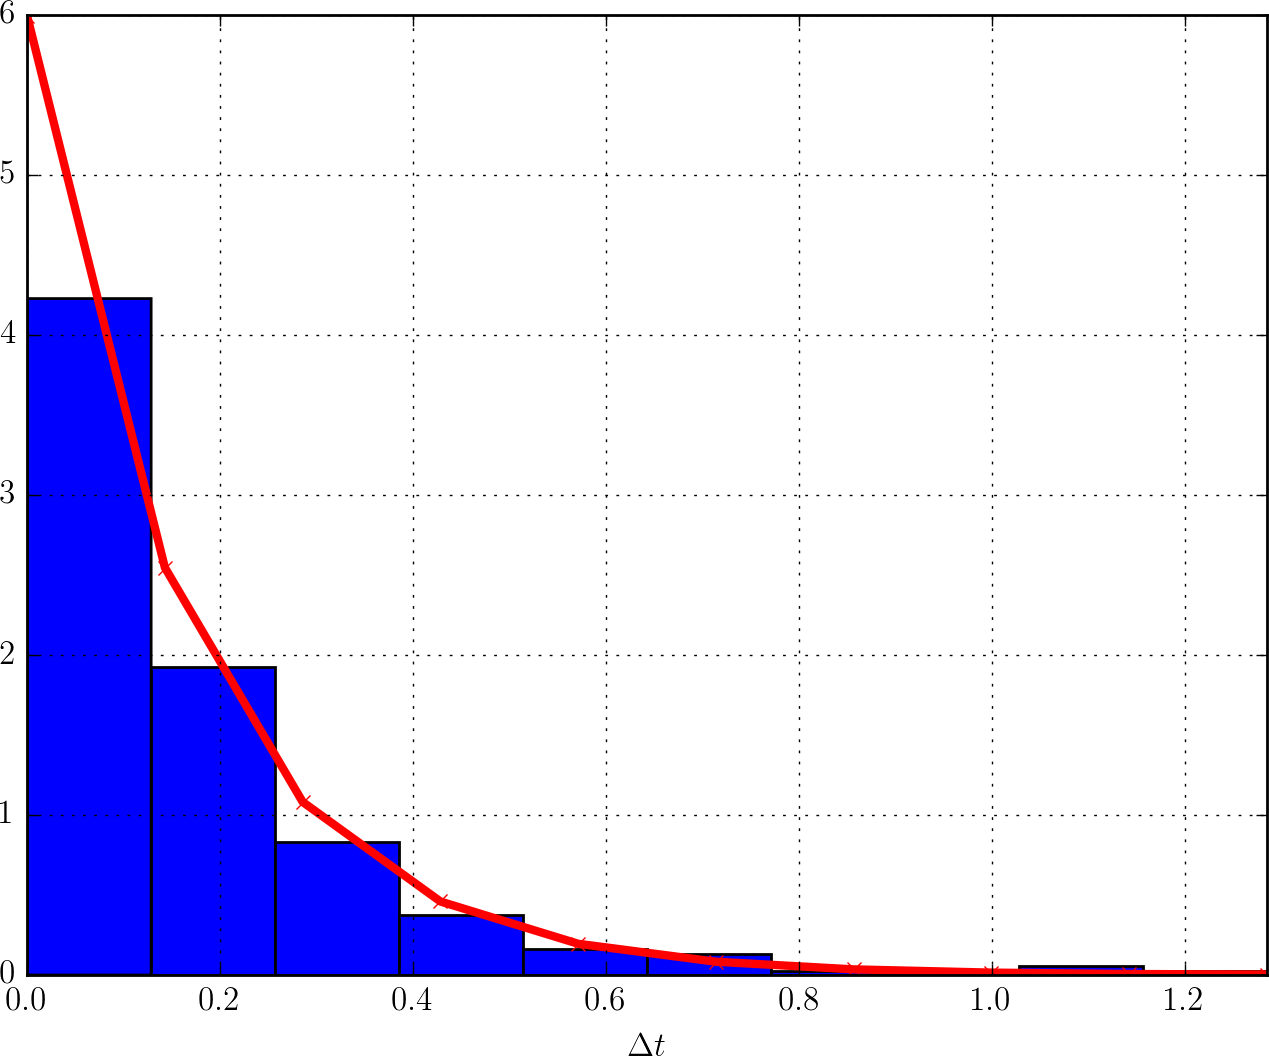
\includegraphics[width=150mm, height=85mm]{pic/hist_2}
  \caption{Гистограмма и плотность вероятности промежутков времени 
    между соседними заявками пуассоновского потока, 
    построенного с помощью алгоритма 2}
  \label{pic:hist_2}
\end{figure}

Оценка параметра $\lambda$ можно найти как математическое ожидание
значений промежутков времени между соседними заявками пуассоновского потока:
\begin{equation*}
  \hat{\lambda} = E[\Delta]^{-1}, \:
  \hat{\lambda}_1 = 5{,}67, \:
  \hat{\lambda}_2 = 5{,}83.
\end{equation*}

Исходный код разработанной программы представлен в приложении~А.